\documentclass[12pt,a4paper]{article}
\usepackage[utf8]{inputenc}
\usepackage{amsmath}
\usepackage{amsfonts}
\usepackage{amssymb}
\usepackage{graphicx}
\author{Iványi Patrik}
\title{Webes alkalmazások fejlesztése - 1. beadandó}

\begin{document}
\maketitle

\section{Feladat}
Készítsük el egy étel-futár vállalat rendeléseket kezelő rendszerét.
\begin{itemize}
\item A weblap főoldalán megjelennek a kategóriák (pl. levesek, pizzák, üdítők),
 valamint a 10 legnépszerűbb (legtöbbet rendelt) étel/ital.
\item A kategóriát kiválasztva listázódnak a tételek (név és ár kíséretében), amelyek szűrhetőek név(részlet)re. Ételek esetén leírás is van. Külön meg vannak jelölve a csípős, illetve vegetáriánus ételek.
\item Ételek és italok tetszőleges számban helyezhetőek a kosárba egy adott felső korlátig (20.000 Ft),  afelett több terméket nem lehet a kosárba helyezni. 
\item A  kosár  tartalma  bármikor  megtekinthető,  ekkor  látszódnak  a felvett tételek, illetve látható az összár. Bármely tétel kivehető a kosárból.
\item A  rendelést törölhetjük,  illetve leadhatjuk.  Utóbbi  esetben meg   kell adnunk a nevünket, címünket, illetve telefonszámunkat, majd elküldhetjük a rendelést.
\end{itemize}

\section{Feladat elemzése}
A feladatot a három rétegű, Model-View-Controller architektúrában valósítjuk meg.
\begin{itemize}
\item Az adatok tárolásához, és a felhasználó kezeléshez létrehozunk egy adatbázist, melyben az ételek/italok, a kategóriák,  a rendeléseket, valamint a vásárlás során a kosár tartalmát téroljuk. Az adatbázis modelljét az RestaurantContext biztosítja.
\item Az oldal egységes megjelenítésért létrehozunk egy megosztott megjelenítőt.
\item A Home könyvtár alatt létrehozzuk a kedvenc ételek/italok listázásért felelős nézetet, valamint az oldalsó menüsávban egy lehetőséget, hogy az adott felhasználó szürhessen kategóriára.
\item Külön nézetet hozunk létre a kategóriák megjelenítése érdekében, a nézet a kiválasztott kategória alapján változtatja tartalmát.
\item A kontrollerek felelőssége csökkentése érdekében létrehozunk két funkcionalitásért felelős osztályt, az AccounstServicet-t, mely a felhasználói műveltekért felelős, valamint az AuctionService-t, amely a konzisztens licitálást biztosítja, valamint a megfelelő licitek és tárgyak elérést biztosítja.
\item A bevásárló kosarat egy ShoppingCart modell segítségével valósítottuk meg, mely az adott session és az adatbázis között épít ki kapcsolatot.
\item Külön kontroller felel a vásárlás lebonyolításáért, valamint az ételek közti keresésekért.
\end{itemize}

\section{Felhasználói estek}
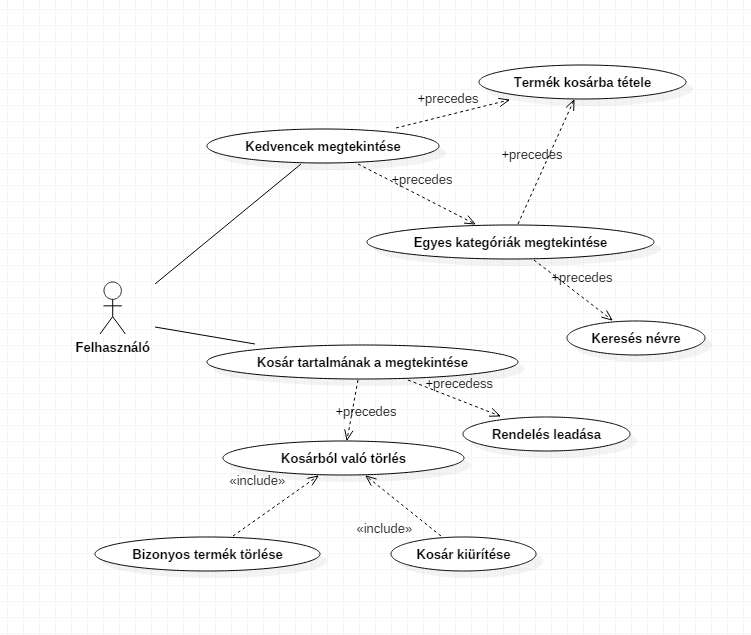
\includegraphics[scale=0.7]{usecase}

\section{A rendszer szerkezete}
\subsection{Komponensek}
Az MVC acthitektúrának megfelelően a programnak 2 fontos komponense van.
\begin{itemize}
\item Az adatbázis felelős a rendszer által használt adatok, és a bevárlás lebonyolításához történő információk tárolására. Az adatbázishoz való kapcsolódást az  Entity Freamwork segítségével biztosítjuk.
\item A webes alkalmazási felület ASP.NET-ben MVC architektúrával megvalósítva, amely tartalmaz felhasználói nézeteket és ehhez kapcsolódó nézetmodelleket, kontrollereket, valamint az adatbázis modelljét, és a funkcionalitásért felelős kiszolgáló osztályokat.

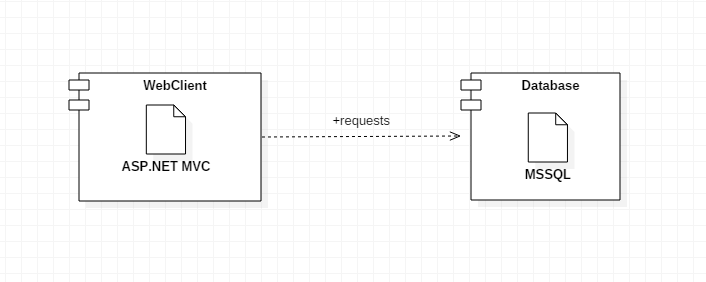
\includegraphics[scale=0.5]{component}

\end{itemize}
\subsection{Osztályok}
\begin{itemize}
\item Külön project felelős az adatbázis modell megvalósításáért, mely kapcsolatban van az alkalmazást megvalósító modellel. 
\item A Models névtéren belül helyezkednek el a nézetmodelleket,  valamint a bevásárlást végző osztályok.
\item A Controllers névtéren belül a kontrollerek helyezkednek el. A program 2 különböző kontrollere oszlik, valamint a közös funkcionalitást biztosító bázis kontrollere.
\item A View-en belül helyezkedik el a közös megjelenítésért felelős nézet, a kedvencek listázásáért felelős főoldali nézet,  a kosár tartalmát megjelenítő és a rendelés leadásáért felelős nézetek, valamint az egyek kategórákhoz tartozó ételek/italokrészleteit megadó felület
\end{itemize}
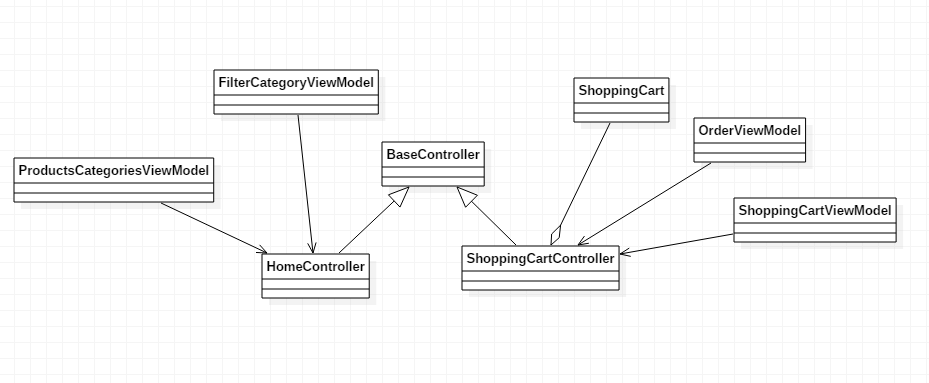
\includegraphics[scale=0.5]{classdiagram}

\section{Adatbázis felépítése}
\begin{itemize}
\item Az adatbázisban tároljuk az egyes ételeket/italokat.
\item A különböző kategóriákat
\item Az adott felhasználó által leadott rendeléseket
\item A bevásárlás lebonyolításához szükséges adatokat
\end{itemize}
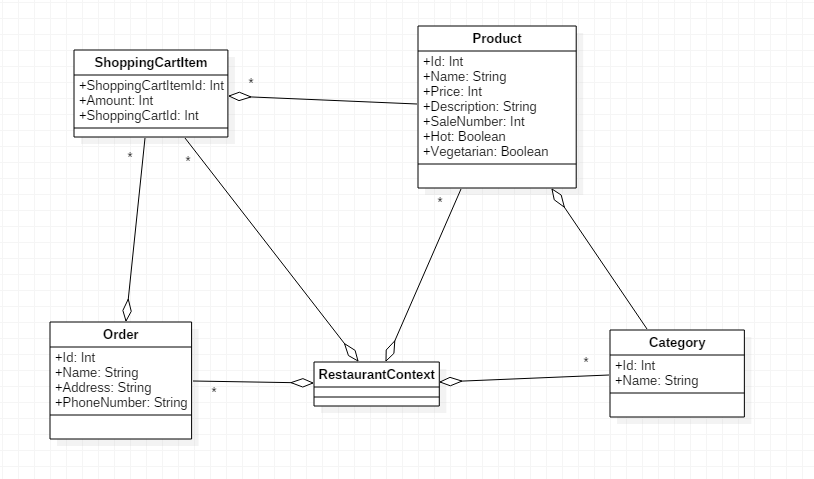
\includegraphics[scale=0.5]{database}

\end{document}